\documentclass[12pt, letterpaper]{article}
\usepackage{graphicx}
\graphicspath{{images/}} 
\usepackage{titling}
\usepackage{amsmath}
\usepackage{listings}
\usepackage{xcolor}
\usepackage{textcomp}
\usepackage{multicol}
\usepackage[utf8]{inputenc}
\usepackage{parallel}
\usepackage{siunitx}
\usepackage{booktabs}
\usepackage{fancyhdr}
\usepackage{tabularx}
\usepackage{caption}
\usepackage[export]{adjustbox}
\usepackage[top=1in, left=0.5in, right=0.5in, bottom=1in]{geometry}
\addtolength{\topmargin}{0in}

\usepackage{libertine}
\renewcommand*\familydefault{\sfdefault}  %% Only if the base font of the document is to be sans serif
\usepackage[T1]{fontenc}







\title{Spatial Mapping System Using Time-of-Flight}
\author{Hamza Siddiqui - 400407170 - siddih38 }
\date{\today}

%\begin{document}

\pagestyle{fancy}

\lhead{Hamza Siddiqui}
%\chead {\today}
\chead {April 16, 2023}
\rhead{SMSUTOF HS 2023 v0.1}


\onecolumn

\begin{figure}
\begin{minipage}{0.47\textwidth}
\centering

\includegraphics[width=.7\textwidth,left,height=.4\textwidth]{logo.png}

\end{minipage}
\hfill
\begin{minipage}{0.47\textwidth}
\raggedleft
\Huge \textbf{Spatial Mapping System using ToF v0.1}
\end{minipage}
\end{figure}


\begin{figure}
\begin{minipage}{0.47\textwidth}

\section*{Core Device Components}
\begin{itemize}
    \item Microcontroller Unit (ARM\textregistered \ Cortex\textregistered-M4F TI MSP432E401Y SimpleLink\texttrademark) 
    \item Stepper Motor (28BYJ-48 Velleman\textregistered\ 5 VDC Stepper Motor with ULN2003 Driver Board)
    \item Time-of-Flight Sensor (ST FlightSense\texttrademark \ VL53L1X)
    \item Additional Push Button 
    \item Removable Sensor Mount (Hamza Electronics\texttrademark)
    \item Fiberboard Case (Hamza Electronics\texttrademark)
\end{itemize}



\end{minipage}
\hfill
\begin{minipage}{0.47\textwidth}
\centering
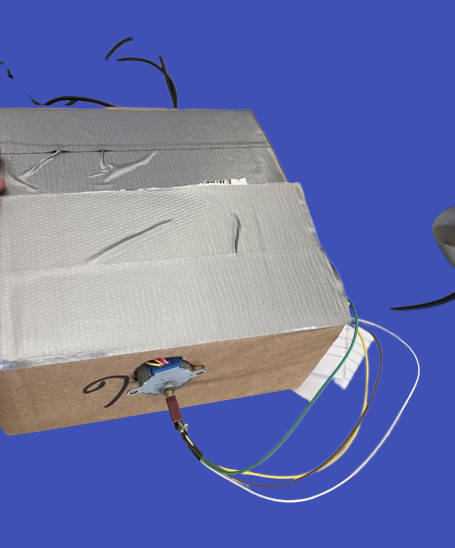
\includegraphics[width=0.7\textwidth,right]{product.png} %PRODUCT IMAGE PLACEHOLDER

\end{minipage}
\end{figure}





\begin{document}
\maketitle
As a future member of the engineering profession, the student is responsible for performing the required work in an honest manner, without plagiarism and cheating.
Submitting this work with my name and student number is a statement and understanding that this work is my own and adheres to the Academic Integrity Policy of McMaster University and the Code of Conduct of the Professional Engineers of Ontario.
\thispagestyle{fancy}

\newpage
\section{Device Overview}
\subsection{Features}
\begin{multicols}{2}
\begin{itemize}
\item ARM Cortex-M4F TI MSP432E401Y Microcontroller (\$53.47)
    \begin{itemize}
        \item Bus frequency of 20MHz (configured via phase-locked loop; default core frequency of 120MHz)
        \item Four onboard LEDs - D3 flash functionality on each measurement
        \item Two onboard buttons (PJ1 for start/stop of motor rotation) and one reset button
        \item 1MB of flash, 256kB of SRAM
        \item  Communication interfaces including USB-OTG, CAN, Quad-SPI (QSSI), $\mathrm{I^2C}$, SPI,  and UART
        \item Two 12-Bit SAR-Based ADC Modules (2 Msps)
    \end{itemize}
\item MOT-28BYJ-48 Stepper Motor with ULN2003 driver (\$6.99)
    \begin{itemize}
        \item 5-12 VDC Operating Range 
        \item 64 steps/revolution 
        \item Frequency of 100Hz
        \item 4 phases with 4 step-indicator LEDs
    \end{itemize}
\item VL53L1X Time-of-Flight Sensor (\$25.32)
    \begin{itemize}
        \item Communication via $\mathrm{I^2C}$ (upto 400kHz)
        \item 4 m ranging and ranging frequency of 50Hz
        \item 2.6-5.5V supply range, 2.8V operating range
        \item Emitter: 940 nm invisible laser (Class1)
    \end{itemize}
\item Additional Push Button (\$0.60)
    \begin{itemize}
        \item Start/stop functionality for data acquisition
    \end{itemize}
\item Additional System Features
    \begin{itemize}
        \item UART serial communication between device and PC
        \item $\mathrm{I^2C}$ serial communication between device and Time-of-Flight sensor
        \item Baud rate of 115200
        \item C-language programming for device instructions, Python programming for visualization (via Pyserial and Open3d)
    \end{itemize}
\end{itemize}
\end{multicols}
\subsection{General Description}
To begin data acquisition, the additional push button is pressed to enable data processing, then the onboard button is pressed to begin taking measurements by spinning the motor and interfacing with the Time-of-Flight (ToF) sensor. The SMSUTOF HS 2023 utilizes a transducer which provides a digital output. Spatial distance measurements are acquired via the ToF sensor using $\mathrm{I^2C}$, while displacement is fixed at 30 cm. At each angle a measurement is taken, the D3 LED flashes. Together these measurements allow the device to measure a 3-D area. These signals are converted to electric signals, then conditioned into digital form and are finally converted to discrete digital values during the ADC process. The system communicates this to the user PC via UART asynchronous serial communication. A Python program is run on the PC and interfaces via their UART COM port and a baud rate of 115200, which then transfers measurement data to the PC and allows it to be stored in a .xyz file. This collected data is then used to generate a 3-D plot of the area that has been scanned via a Python program using open3d. The points for this plot are generated using trigonometric properties based on the angle and y,z coordinates generated, along with the fixed x-coordinate increment. If at anytime the button is pressed again during the scanning process, the data acquisition will be stopped. 
\subsection{Block Diagram (Data Flow Graph)}
\begin{figure}[h]
    \centering
    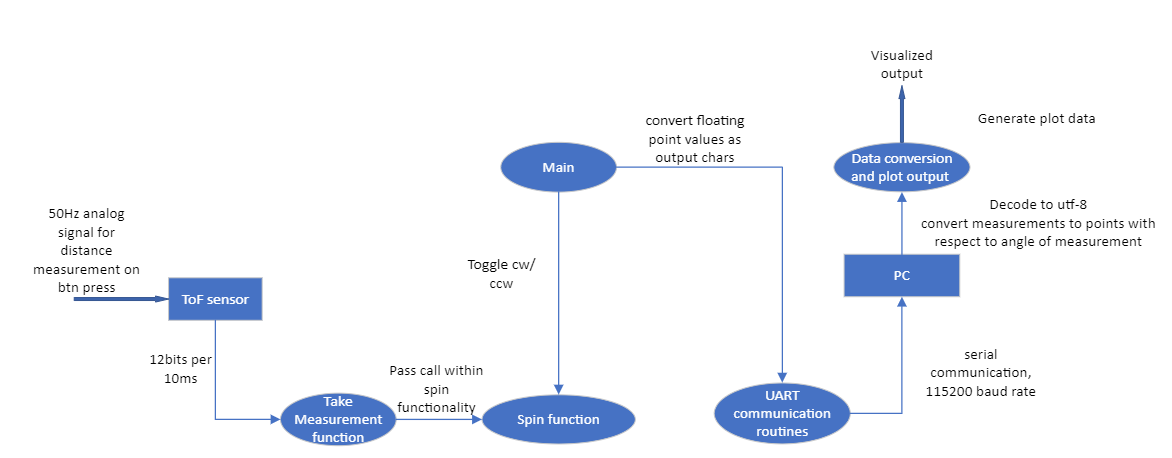
\includegraphics[width=\textwidth]{images/flowgraph.png}
    \caption{Flow graph}
    \label{fig:flowgraph}
\end{figure}

\section{Device Characteristics Table}
\begin{center}
\begin{tabularx}{0.5\textwidth}{|>{\centering\arraybackslash}X|>{\centering\arraybackslash}X|>{\centering\arraybackslash}X|}
\hline
\textbf{Characteristic} & \textbf{Description} \\
\hline
Bus Speed & 20MHz \\
\hline
Serial Port & COM4 \\
\hline
Communication Speed & 115200 bps \\
\hline
Measurement Status & D3 \\
\hline
\end{tabularx}
\captionof{table}{Device Characteristics}
\end{center}

\begin{minipage}{0.48\textwidth}
\centering
\textbf{Stepper Motor Pin Assignments}
\begin{tabular}{|c|c|}
\hline
\textbf{ULN2003 Driver Board} & \textbf{MCU} \\
\hline
+ (5V) & 5V \\
\hline
- (5V) & GND \\
\hline
IN1 & PH0 \\
\hline
IN2 & PH1 \\
\hline
IN3 & PH2 \\
\hline
IN4 & PH3 \\
\hline
\end{tabular}
\captionof{table}{Stepper Motor Pinout}
\end{minipage}
\hfill
\begin{minipage}{0.48\textwidth}
\centering
\textbf{Time-of-Flight Sensor Pin Assignments}
\begin{tabular}{|c|c|}
\hline
\textbf{VL53L1X} & \textbf{MCU} \\
\hline
VDD & - \\
\hline
VIN & VCC (3.3V or 5V) \\
\hline
GND & GND \\
\hline
SDA & PB3 (I2C0 SDA) \\
\hline
SCL & PB2 (I2C0 SCL)  \\
\hline
XSHUT & - \\
\hline
GPIO1 & - \\
\hline
\end{tabular}
\captionof{table}{Time-of-Flight Sensor Pinout}
\end{minipage}


\section{Detailed Description}
\subsection{Distance Measurement}
\textbf{Acquisition:}\\
The VL53L1X sensor utilizes Light Detection and Ranging (LIDAR) technology to accurately measure distances. It emits a pulse of light with a wavelength of 940 nm, which is then reflected back to the sensor by an object (maximum 4 m away). The sensor measures the time it takes for the emitted light pulse to reach the object and be reflected back to the detector. By utilizing the known speed of light and the measured time, the VL53L1X calculates the distance to the object with high accuracy as follows:
$$Measured\ Distance = \frac{Photon\ Travel\ Time}{2}\times Speed\ of\ Light$$ The sensor is mounted to a motor that completes 360 degree rotations (512 steps). At every 64 steps, or 45 degrees, a user LED is flashed to indicate a measurement (in mm) has been taken by the sensor. This is achieved through interfacing with the sensor and micro controller via $\mathrm{I^2C}$ serial communication. In total, this allows for 8 measurements to be taken in a single rotation, and the program can be modified to measure at smaller number of steps to take more measurements for more accuracy at the cost of time (use-case dependent configuration). \\ 
\textbf{Data Processing:} \\
Data is processed and converted via mathematical computation. When given the motor's angle $\theta$, the program increments by the measurement angle rotation each time and computes the coordinates using trigonometric properties. This is computed as $angle = steps/(TOTAL STEPS) \times 2\pi$ where steps is incremented by 45 degrees and TOTAL STEPS is set to 512 - these reset each time a rotation is complete i.e. when 512 steps have completed. For a given distance measurement $r$, we obtain that $y = r\cos{\theta}$ and $z = r\sin{\theta}$ for the vertical plane. X coordinate is computed through configuring a physical step increment taken for each successive measurement rotation in the program and incrementing the coordinate for the next spatial scan based on this value (350mm default configuration). Together these coordinates can be used for plotting and mapping. 




\subsection{Visualization}
\section{Application Example with Expected Output}
\section{User's Guide}
\section{Limitations}
\section{Circuit Schematic}
\section{Programming Logic Flowchart(s)}


\end{document}